\section{\bench{} 基准及其有效性审计}
\label{sec:benchmark}

\subsection{场景、机器人与传感}
\bench{} 基于 ManiSkill3\cite{tao2025maniskill3}构建。每个回合随机生成一棵带主干、枝条和叶簇的果树，挂有 4--6 颗半径 2.5--2.9~cm 的球形果实，果实高度 0.44--0.64~m，距机器人基座 0.38--0.50~m，方位角在 $\pm28^\circ$ 以内。布局采样器保证每颗果实都存在水平接近的逆运动学解、接近通道内没有枝条，且果实在前置相机中互不遮挡。果实被双指连续夹持 2 个控制步后脱离果柄，成为自由刚体。机器人为睿尔曼 RM75-B 七自由度机械臂加 EG2 两指夹爪，关节位置控制，控制频率 20~Hz。观测包括前置和腕部两台 RGB-D 相机（$256\times256$ 像素，前置视场角 $55^\circ$，腕部 $90^\circ$）以及 8 维本体状态（7 个关节角和 1 个夹爪开度）。集果篮位于机器人侧方，始终在前置相机视野之外。图~\ref{fig:scene} 为真实渲染画面。

\begin{figure}[t]
\centering
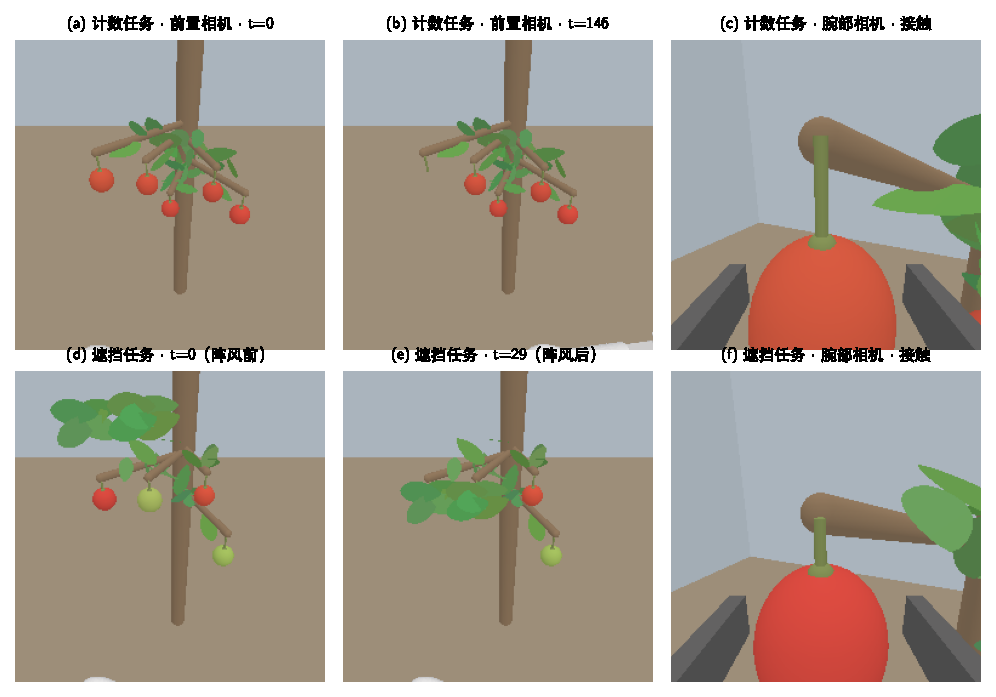
\includegraphics[width=0.86\linewidth]{zh_scene}
\caption{\bench{} 场景（真实渲染，v1 任务）。(a)--(c) 计数任务：开始时与一次采摘后的前置相机画面，以及接触时刻的腕部画面；(d)--(f) 遮挡任务：阵风前后的前置相机画面（阵风后两个叶簇遮住果实）以及接触时刻的腕部画面。v2 任务在此基础上增加风落果和颜色褪变（图~\ref{fig:tasks}）。}
\label{fig:scene}
\end{figure}

\subsection{原始任务为何检测不出记忆差异}
\label{sec:v1}
基准的第一版（v1）包含两个任务。\textbf{计数任务}要求在 $M$ 颗成熟果中恰好摘 $N$ 颗（$N=2$--5），入篮数达到 $N$ 即判成功。\textbf{遮挡任务}中红果与青果混挂，观察阶段第 8--20 步的一阵风把两个叶簇吹到两颗果实前方，指令要求把所有成熟果放入篮中、不放青果。按设计，前者需要记住自己摘了几颗，后者需要记住被遮住的果实是否成熟。

我们按预先登记的协议，在 val 50--99 布局 $\times$ 3 个种子（每格 \V{v1_n} 次）上比较了 K0（均匀记忆）与 K4、K8（平坦事件关键帧 \pekm{}，几何事件）三种策略。结果如表~\ref{tab:v1} 所示：四项主假设均未获支持，Holm 校正后 $p=\V{v1_holm}$。事后诊断找到了三个原因：
\begin{enumerate}
\item \textbf{计数任务在达到配额时自动结束。}仿真环境在成功或失败时立即终止回合，入篮数一旦等于 $N$ 就判成功，策略根本没有“多摘”的机会；这类记忆失败在结构上恒为 \V{v1_cnt_memfail}。
\item \textbf{遮挡任务可以靠当前画面完成。}叶簇本身标出了被遮果实的位置，被遮果实中 \pct{v1_hidden_ripe_frac} 是成熟的；更关键的是，叶片在 TCP 进入 15~cm 范围时会被推开，K0 接近被遮挡成熟果时有 \pct{v1_leaf_lift} 的情况叶片抬起、露出果实颜色。策略只需“走近看一眼”。
\item \textbf{场景信息天然被均匀记忆保留。}均匀采样总是包含第 0 帧，阵风前的画面在三种记忆的所有决策中都被保留（\pct{v1_frame0}），因此三者在场景信息上没有差别；在推理时去掉阵风前的帧，遮挡任务成功率仅从 \pct{v1_nopregust_a} 降到 \pct{v1_nopregust_b}。
\end{enumerate}
结论是：v1 的零结果说明这个基准检测不出记忆差异，而不能说明事件关键帧无效。这一教训促使我们在评估任何记忆方法之前，先审计任务是否真的需要记忆。

\begin{table}[t]
\centering
\caption{v1 原始任务上的预登记正式评测（真实结果；每格 150 次，val 50--99 $\times$ 种子 7/8/9）}
\label{tab:v1}
\small
\begin{tabular}{lcccl}
\toprule
任务 & K0 均匀 & K4 & K8 & 诊断\\
\midrule
计数（v1） & \pct{v1_cnt_k0} & \pct{v1_cnt_k4} & \pct{v1_cnt_k8} & 达到配额即终止，多摘失败结构性为 0\\
遮挡（v1） & \pct{v1_occ_k0} & \pct{v1_occ_k4} & \pct{v1_occ_k8} & 叶片靠近即抬起，颜色可见\\
遮挡错果率 & \pct{v1_occ_wrong_k0} & \pct{v1_occ_wrong_k4} & \pct{v1_occ_wrong_k8} & 第 0 帧在所有决策中均被保留\\
\bottomrule
\end{tabular}
\end{table}

\subsection{v2 任务：把场景记忆与事件记忆分开}
\label{sec:tasks}
v2 的设计目标有三条：无记忆策略的成功率必须很低；场景记忆与事件记忆分开检验，并把预测事先写入协议；事件数量要足够多，能够检验记忆容量（图~\ref{fig:tasks}）。

\textbf{计数 v2（事件记忆）。}取消“入篮数等于 $N$ 即结束”。回合在以下任一情况结束：策略发出\emph{完成信号}（回到休息位姿附近、夹爪张开、未持果，且静止至少 40 步）；达到步数预算；入篮数超过 $N$（立即判失败）；机器人掉果（立即判失败）。成功定义为结束时入篮数恰好为 $N$ 且没有掉果。为堵住“开头数总果数 $M$、当前数剩余果数 $R$、用 $M-R$ 推算已摘数”的捷径，回合中途会随机让 1--2 颗未被摘取的果实被风吹落到地面；风落果单独标记，不算机器人掉果，也不会落入篮中。于是“已摘几颗”只存在于机器人自己每次放果的短暂时刻中，这正是事件记忆的情形。专家在放完第 $N$ 颗后回到休息位姿并保持静止。

\textbf{遮挡 v2（场景记忆）。}阵风期间（第 8--20 步），所有果实的外观颜色逐渐褪变为同一种中性色，两台相机此后都无法再分辨成熟度，成熟度信息只存在于阵风前的画面中；叶簇保留。成功定义不变：所有成熟果入篮，且没有青果入篮。由于均匀记忆总是保留第 0 帧，而 \hem{} 的场景锚层同样保留第 0 帧，我们\emph{预测}该任务上各记忆条件之间没有差异。这一任务用作“不伤害场景记忆”的等效性检验。

\textbf{多株长时配额 FruitRow（长时事件记忆）。}模拟沿种植行连续作业的场景：一行 3 株植物，每株挂 3--5 颗成熟果和若干青果，指令要求整行共摘 $N$ 颗成熟果（$N=6$--12）。当前株已无可摘成熟果时，平台把下一株移到机器人前方（仿真中替换场景并发出换株信号），此前的植株随即离开视野。风落果机制与计数 v2 相同，回合同样由完成信号结束。平均每回合 \V{row_events} 次采摘、\V{row_steps} 个控制步，远超平坦事件关键帧的容量。由于前面植株上的采摘既不可见、也无法从当前株推算，记住整行的累计采摘次数只能依靠长时事件记忆。

\begin{figure}[t]
\centering
\resizebox{\linewidth}{!}{%
\begin{tikzpicture}[font=\footnotesize, x=0.0103cm, y=1cm]
\def\L{1000}
% count v2
\node[anchor=east, align=right] at (-20,0) {\textbf{计数 v2}\\事件记忆};
\draw[thick,-{Stealth}] (0,0) -- (\L,0);
\fill[gray!25] (0,-0.18) rectangle (30*2.2,0.18);
\node[above] at (33,0.18) {观察};
\foreach \x/\n in {190/1,390/2,600/3}{
  \fill[blue!60] (\x,-0.18) rectangle (\x+14,0.18);
  \node[above, text=blue!60!black] at (\x+7,0.18) {放果 \n};
}
\foreach \x in {300,520}{
  \draw[red!70!black, thick] (\x,-0.32) -- (\x,0.32);
  \node[below, text=red!70!black] at (\x,-0.3) {风落果};
}
\fill[green!50!black!50] (760,-0.18) rectangle (900,0.18);
\node[above, text=green!40!black] at (830,0.18) {完成信号（静止 $\ge$40 步）};
\node[anchor=west, align=left, text=gray!40!black] at (1010,0) {篮子不在前置视野；\\$M-R\neq$ 已摘数};
% occluded v2
\node[anchor=east, align=right] at (-20,-1.25) {\textbf{遮挡 v2}\\场景记忆};
\draw[thick,-{Stealth}] (0,-1.25) -- (\L,-1.25);
\shade[left color=red!60, right color=gray!50] (8*2.2,-1.43) rectangle (20*2.2,-1.07);
\fill[gray!25] (0,-1.43) rectangle (8*2.2,-1.07);
\fill[gray!25] (20*2.2,-1.43) rectangle (30*2.2,-1.07);
\node[above] at (33,-1.07) {阵风+褪色};
\foreach \x/\n in {200/1,430/2}{
  \fill[blue!60] (\x,-1.43) rectangle (\x+14,-1.07);
  \node[above, text=blue!60!black] at (\x+7,-1.07) {采摘 \n};
}
\fill[gray!50] (66,-1.55) rectangle (\L,-1.5);
\node[below, text=gray!40!black] at (520,-1.5) {此后所有果实为同一中性色，成熟度只存在于阵风前画面};
\node[anchor=west, align=left, text=gray!40!black] at (1010,-1.25) {均匀记忆与场景锚均保留第 0 帧；\\预测各记忆条件无差异};
% FruitRow
\node[anchor=east, align=right] at (-20,-2.6) {\textbf{FruitRow}\\长时事件记忆};
\draw[thick,-{Stealth}] (0,-2.6) -- (\L,-2.6);
\foreach \a/\b/\n in {0/330/1,345/665/2,680/985/3}{
  \fill[green!12] (\a,-2.78) rectangle (\b,-2.42);
  \node[above, text=green!35!black] at ({(\a+\b)/2},-2.42) {第 \n 株};
}
\foreach \x in {337,672}{ \draw[black!70, very thick, densely dashed] (\x,-2.86) -- (\x,-2.34); }
\node[below, text=black!60] at (504,-2.86) {换株：前面植株离开视野};
\foreach \x in {60,120,190,255,400,470,540,610,730,800}{ \fill[blue!60] (\x,-2.78) rectangle (\x+10,-2.42); }
\draw[red!70!black, thick] (430,-2.92) -- (430,-2.28);
\fill[green!50!black!50] (880,-2.78) rectangle (970,-2.42);
\node[anchor=west, align=left, text=gray!40!black] at (1010,-2.6) {平均 \V{row_events} 次采摘；\\超出平坦关键帧容量};
\draw[-{Stealth}] (0,-3.45) -- (150,-3.45) node[right] {控制步（示意）};
\end{tikzpicture}}
\caption{v2 三个任务的时间结构（示意）。计数 v2 中，回合由策略的完成信号结束，中途的风落果使“开头果数减当前果数”不再等于已摘数；遮挡 v2 中，阵风期间颜色褪变，成熟度只存在于开头画面中；FruitRow 中采摘分布在 3 株植物上，换株后前面植株离开视野，时间轴按比例压缩。}
\label{fig:tasks}
\end{figure}

\subsection{信息受限脚本策略的捷径审计}
\label{sec:audit}
为检验任务是否真的需要相应的记忆，我们构造三种基于真值的脚本策略，它们使用相同的专家运动规划，只是能用于\emph{决策}的信息不同：(O1) 只用当前帧可见的信息；(O2) 第 0 帧加当前帧；(O3) 完整历史，即专家本身。每个任务每种策略各在 \V{audit_n} 个 dev 布局上运行。事先规定的通过标准是：计数 v2 与 FruitRow 中 O1 和 O2 的成功率都不高于 30\%，O3 不低于 90\%（FruitRow 的 O2 使用当前株的第一帧）；遮挡 v2 中 O1 不高于 30\%，O2 和 O3 都不低于 90\%（场景记忆按设计只需第 0 帧）。此外要求专家逐尝试成功率不低于 90\%，示范通过安全包络时的裁剪率低于 0.5\%。

审计结果见表~\ref{tab:audit}，三个任务均达到预设标准。计数 v2 中，只看当前帧的策略无从知道已摘几颗，典型失败是持续采摘直到超额；看第 0 帧的策略会用 $M-R$ 估计已摘数，被风落果误导，典型失败为少摘后提前发出完成信号。遮挡 v2 中，只看当前帧的策略只能在同色果实间猜测成熟度，成功率接近随机猜测水平；只要能看到第 0 帧，成功率就与完整历史相当。FruitRow 上 O1、O2 几乎全部失败，因为前面植株上的采摘无从推算。这说明计数 v2 与 FruitRow 检验的是事件记忆，遮挡 v2 检验的是场景记忆，与设计一致。

事件信号本身也需要审计。v1 中的几何事件只计算到“成熟且仍挂树”的果实的距离，用到了成熟度真值，可能通过选帧间接向策略提示成熟度。v2 中我们统一采用第~\ref{sec:event_def} 节与成熟度无关的物理事件定义，训练与评测的所有记忆条件使用同一定义。

\begin{table}[t]
\centering
\caption{v2 任务的捷径审计（每格 \V{audit_n} 个 dev 布局）}
\label{tab:audit}
\small
\setlength{\tabcolsep}{3pt}
\begin{tabular}{lcccl}
\toprule
任务 & O1 仅当前帧 & O2 首帧+当前帧 & O3 完整历史 & 预设标准\\
\midrule
计数 v2（事件记忆） & \pct{aud_cnt_o1} & \pct{aud_cnt_o2} & \pct{aud_cnt_o3} & O1、O2 $\le$30\%；O3 $\ge$90\%\\
遮挡 v2（场景记忆） & \pct{aud_occ_o1} & \pct{aud_occ_o2} & \pct{aud_occ_o3} & O1 $\le$30\%；O2、O3 $\ge$90\%\\
FruitRow（长时事件记忆） & \pct{aud_row_o1} & \pct{aud_row_o2} & \pct{aud_row_o3} & O1、O2 $\le$30\%；O3 $\ge$90\%\\
\midrule
\multicolumn{5}{l}{专家逐尝试成功率（计数 v2 / 遮挡 v2 / FruitRow）：\pct{exp_cnt} / \pct{exp_occ} / \pct{exp_row}；示范裁剪率：\pct{clip_cnt} / \pct{clip_occ}}\\
\bottomrule
\end{tabular}
\end{table}
